\documentclass[crop]{standalone}

\usepackage{tikz}
\usetikzlibrary{trees,calc}
\begin{document}

\tikzstyle{every node}=[draw=black,thick,anchor=west]
\tikzstyle{grayed node}=[draw=black!60,text=black!60,dashed]

%\small
\sffamily

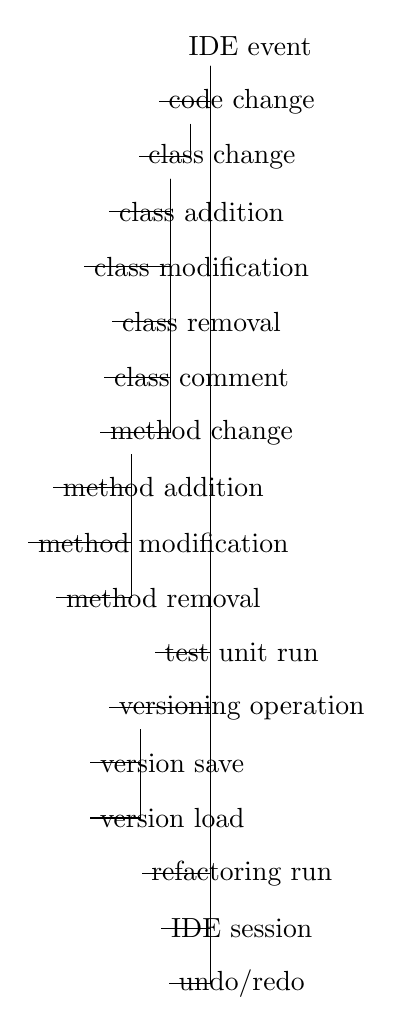
\begin{tikzpicture}[%
    grow via three points={
        one child at (0.8,-0.7) and two children at (0.8,-0.7) and (0.8,-1.4)
    },
    edge from parent path={
        ($(\tikzparentnode\tikzparentanchor)+(.4cm,0pt)$) |- (\tikzchildnode\tikzchildanchor)
    },
    growth parent anchor=west,
    parent anchor=south west]
  \node {IDE event}
    child { node {code change}
    child { node {class change}
      child { node {class addition}}
      child { node {class modification}}
      child { node {class removal}}
      child { node {class comment}}
      child { node {method change}
        child { node {method addition}}
        child { node {method modification}}
        child { node {method removal}}
      }
    }
    child [missing] {}
    child [missing] {}
    child [missing] {}
    child [missing] {}
    child [missing] {}
    child [missing] {}
    child [missing] {}
    child [missing] {}
    child [missing] {}
    child [missing] {}
    }
    child [missing] {}
    child [missing] {}
    child [missing] {}
    child [missing] {}
    child [missing] {}
    child [missing] {}
    child [missing] {}
    child [missing] {}
    child [missing] {}
    child { node {test unit run}}
    child { node {versioning operation}
      child { node {version save}}
      child { node {version load}}
    }
    child [missing] {}
    child [missing] {}
    child { node {refactoring run}}
    child { node {IDE session}}
    child { node {undo/redo}}
    child [missing] {};
\end{tikzpicture}

\end{document}

%\MC & save, load \\

%%% Local Variables:
%%% mode: latex
%%% TeX-master: t
%%% End:
